\documentclass[conference]{IEEEtran}
\IEEEoverridecommandlockouts

\usepackage{amsmath,amssymb,amsfonts}
\usepackage{algorithmic}
\usepackage{graphicx}
\usepackage{textcomp}
\usepackage{xcolor}
\usepackage{booktabs}
\usepackage{multirow}
\usepackage{url}
\usepackage{cite}
\usepackage{balance}

\def\BibTeX{{\rm B\kern-.05em{\sc i\kern-.025em b}\kern-.08em
    T\kern-.1667em\lower.7ex\hbox{E}\kern-.125emX}}

\begin{document}

\title{Cross-Lingual Audio Deepfake Detection: Sensitive Layer Summarization on Frozen XLS-R for Low-Resource Hindi Speech}

\author{\IEEEauthorblockN{Anonymous Authors}
\IEEEauthorblockA{\textit{Department of Computer Science and Engineering} \\
\textit{Research Track Submission}\\
Email: author@institution.edu}
}

\maketitle

\begin{abstract}
Recent advances in neural voice cloning and text-to-speech synthesis (TTS) have made audio deepfakes an alarming threat to societal security, particularly in non-English linguistic regions where dedicated spoofing benchmarks and language-specific detectors are scarce. In this paper, we investigate the cross-lingual generalization and parameter-efficient adaptation of \textbf{Sensitive Layer Summarization (SLS)} on top of a frozen multilingual foundation model (\textbf{Wav2Vec2 XLS-R 300M}) for Hindi speech deepfake detection. 

We uncover a critical methodological pitfall in cross-lingual benchmarking: \textit{generator acoustic bias}. When evaluated on single-source synthetic audio (V1), detectors exploit spurious vocoder shortcuts, yielding an artificially low Equal Error Rate (EER) of \textbf{0.40\%}. To eliminate this shortcut, we construct a strictly balanced, multi-generator benchmark (V2) comprising 400 test samples (200 bonafide from studio and crowdsourced recordings; 200 spoof evenly stratified across 5 distinct TTS architectures: Edge-TTS, FastSpeech, Indic-TTS, VITS-MMS, and XTTS-v2). 

Evaluating an English-pretrained SLS checkpoint zero-shot on Hindi reveals a substantial cross-lingual domain shift: genuine Hindi speech is recognized with 98.00\% recall, but synthetic speech frequently escapes detection, resulting in an EER of \textbf{28.90\%} and an accuracy of \textbf{60.00\%}. Fine-tuning only the lightweight SLS classifier head ($\sim$22.8M parameters) with few-shot Hindi supervision rapidly bridges this gap: with as few as $N=10$ samples per class, EER improves to \textbf{26.88\%} ($65.83\%$ accuracy); scaling to $N=50$ samples per class reduces EER to \textbf{19.70\%} and drives accuracy to \textbf{79.67\%} (a 9.2\% absolute EER reduction). 

Furthermore, we conduct an architectural ablation on an NVIDIA L4 GPU to examine whether fine-tuning transformer backbone layers benefits cross-lingual adaptation. Unfreezing the top 2 layers degrades EER to \textbf{24.14\%}, and unfreezing the top 4 layers leads to catastrophic few-shot overfitting (\textbf{25.31\% EER}, $67.12\%$ accuracy). Our empirical findings demonstrate that keeping 100\% of the multilingual foundation backbone frozen is decisively superior under few-shot data regimes ($N \le 50$), validating the parameter-efficient SLS paradigm for cross-lingual deepfake defense.
\end{abstract}

\begin{IEEEkeywords}
Audio deepfake detection, cross-lingual transfer, foundation models, XLS-R, selective layer summarization, few-shot learning, dataset bias.
\end{IEEEkeywords}

\section{Introduction}
Synthetic speech generated via modern diffusion, flow-matching, and neural vocoder architectures has made high-fidelity voice cloning accessible at consumer scale \cite{wang2022comparative}. While deepfake detectors trained on established English corpora (e.g., ASVspoof 2019/2021 \cite{yamagishi2021asvspoof}) achieve sub-1\% Equal Error Rates (EER) in in-domain conditions, deployment in real-world scenarios requires robust cross-lingual generalization.

The vast majority of synthetic speech research remains concentrated on English. Indic languages such as Hindi---spoken by over 600 million people worldwide---remain severely underserved by defensive technologies. Deploying English-trained detection models directly on Hindi audio exposes populations to high false-acceptance vulnerabilities, creating substantial risks in telephonic fraud, financial voice-authorization scams, and political disinformation.

Building dedicated large-scale deepfake datasets for every under-resourced language is economically and computationally prohibitive. Consequently, a vital research question arises: \textit{Can a deepfake detection head pretrained on high-resource English transfer to an under-resourced target language with minimal supervision, and what architectural constraints govern this transfer?}

This work provides a rigorous investigation into this question using the \textbf{Selective / Sensitive Layer Summarization (SLS)} framework \cite{zhang2024sensitive} built on a frozen \textbf{XLS-R 300M} foundation model \cite{babu2022xls}. Specifically, our contributions are:

\begin{enumerate}
    \item \textbf{Quantifying Cross-Lingual Domain Shift}: We evaluate an English-pretrained SLS detector on Hindi speech without target-language adaptation (Zero-Shot), demonstrating an asymmetric failure mode where genuine speech is preserved (98.00\% recall) while 44.3\% of synthetic speech evades detection (28.90\% EER).
    \item \textbf{Uncovering and Resolving Generator Bias}: We demonstrate that evaluating synthetic speech detectors on unstratified datasets (V1) creates spurious correlation shortcuts, artificially deflating EER to 0.40\%. We formalize a 5-generator stratified evaluation protocol (V2) that prevents acoustic shortcut learning and measures true cross-generator generalization.
    \item \textbf{Parameter-Efficient Few-Shot Adaptation}: We show that fine-tuning solely the lightweight SLS head with $N \in \{10, 50\}$ Hindi samples per class achieves monotonic performance gains, decreasing EER from 28.90\% to 19.70\% and increasing accuracy from 60.00\% to 79.67\%.
    \item \textbf{Backbone Unfreezing vs. Frozen Foundation Analysis}: On an NVIDIA L4 GPU, we show that unfreezing transformer backbone layers during few-shot adaptation causes severe overfitting, confirming that keeping the 315M-parameter foundation backbone completely frozen provides optimal regularization.
\end{enumerate}

\begin{figure}[t]
\centering
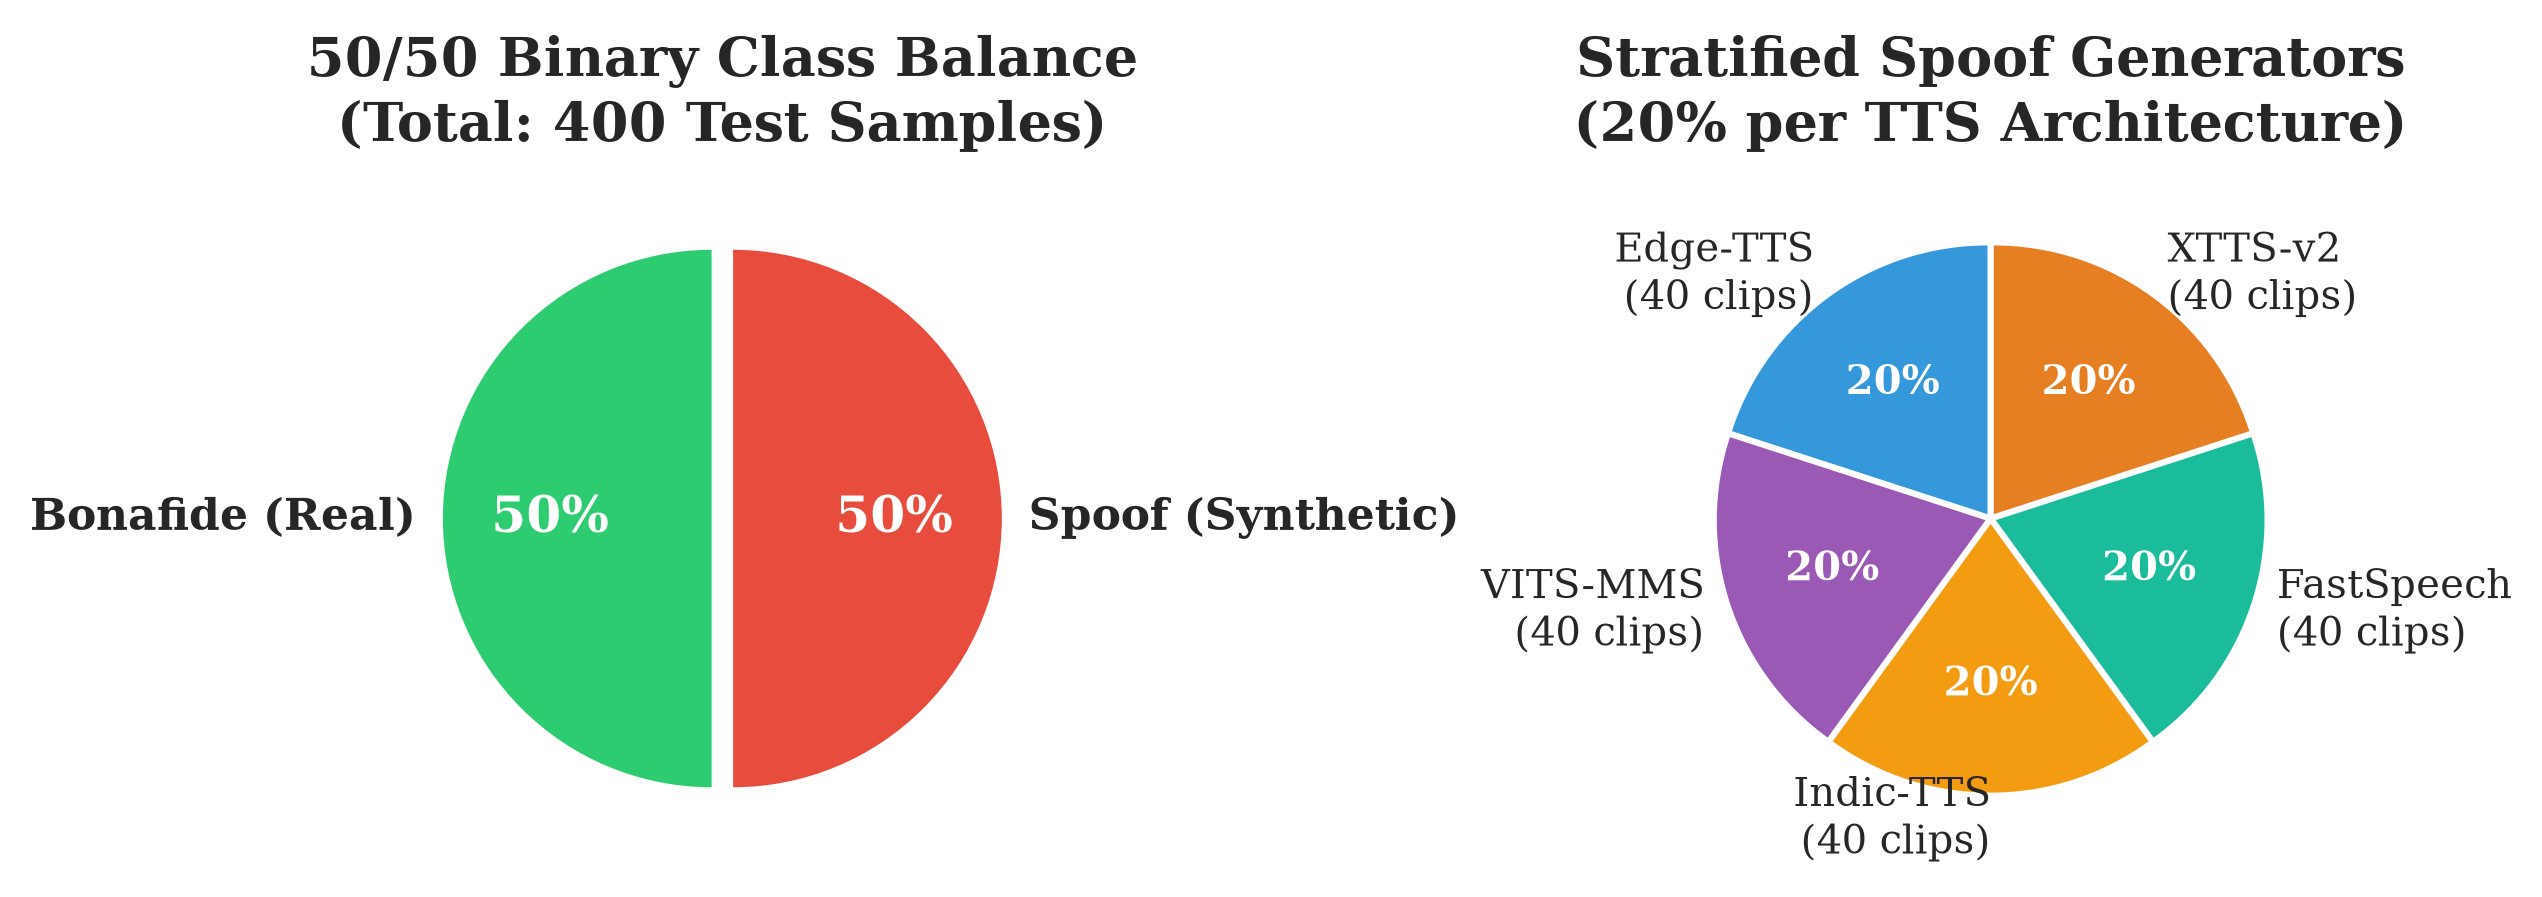
\includegraphics[width=\columnwidth]{../outputs/figures/fig4_generator_stratification.png}
\caption{Architecture of the V2 Balanced Benchmark: 50/50 Binary Class Balance (left) and strict 20\% stratification across 5 distinct TTS generator architectures (right).}
\label{fig:generator_stratification}
\end{figure}

\section{Methodology \& Architecture}

\subsection{Multilingual Foundation Backbone (XLS-R 300M)}
We employ \textbf{Wav2Vec2 XLS-R 300M} (\texttt{facebook/wav2vec2-xls-r-300m}), trained on 436,000 hours of unlabelled speech spanning 128 languages \cite{babu2022xls}.
\begin{itemize}
    \item \textbf{Input Preprocessing}: Raw audio waveforms sampled at 16 kHz are standardized to a fixed length $L = 64{,}600$ samples ($\sim$4.04 seconds). Shorter utterances are tile-padded; longer utterances are center-cropped.
    \item \textbf{Latent Feature Extraction}: A 7-block temporal convolutional feature encoder transforms the raw audio into latent feature vectors.
    \item \textbf{Transformer Representations}: The 24-layer transformer encoder produces hidden representations:
    \begin{equation}
        H_l \in \mathbb{R}^{B \times T \times 1024}, \quad l \in \{1, 2, \dots, 24\}, \quad T = 201
    \end{equation}
    \item \textbf{Freezing Constraint}: The entire backbone parameter set $\Theta_{\text{backbone}}$ is kept frozen ($\nabla_{\Theta_{\text{backbone}}} = 0$) during standard few-shot training.
\end{itemize}

\subsection{Sensitive Layer Summarization (SLS) Head}
Traditional audio classifiers often attach a classification head solely to the final (24th) transformer layer. However, synthetic audio artifacts---such as vocoder phase discontinuity, high-frequency harmonic distortion, and pitch modulation collapse---manifest across intermediate depths of the transformer hierarchy, whereas top layers encode linguistic abstractions \cite{zhang2024sensitive}.

SLS addresses this by learning a per-layer attention gating mechanism over all 24 transformer representations:
\begin{enumerate}
    \item \textbf{Per-Layer Gating}: Each layer's representation $H_l$ is temporally average-pooled:
    \begin{equation}
        \bar{h}_l = \frac{1}{T} \sum_{t=1}^T H_l[:, t, :] \in \mathbb{R}^{B \times 1024}
    \end{equation}
    and projected through a learned linear transformation with sigmoid activation:
    \begin{equation}
        \alpha_l = \sigma(W_0 \bar{h}_l + b_0) \in \mathbb{R}^{B \times 1}, \quad W_0 \in \mathbb{R}^{1024 \times 1}
    \end{equation}
    \item \textbf{Dynamic Layer Fusion}:
    \begin{equation}
        H_{\text{fused}} = \sum_{l=1}^{24} \alpha_l \odot H_l \in \mathbb{R}^{B \times T \times 1024}
    \end{equation}
    \item \textbf{2D Downsampling Block}: Treating $H_{\text{fused}}$ as a single-channel 2D feature map of shape $(B, 1, T, 1024)$:
    \begin{equation}
        Z = \text{MaxPool2D}(\text{SELU}(\text{BatchNorm2D}(H_{\text{fused}})))
    \end{equation}
    with kernel size $(3, 3)$ and stride $(3, 3)$, yielding a flattened feature representation $z \in \mathbb{R}^{B \times 22847}$.
    \item \textbf{Classifier MLP}:
    \begin{equation}
        \hat{y} = \text{LogSoftmax}(W_3 \cdot \text{SELU}(W_1 z + b_1) + b_3)
    \end{equation}
    where $W_1 \in \mathbb{R}^{22847 \times 1024}$ and $W_3 \in \mathbb{R}^{1024 \times 2}$.
\end{enumerate}

\subsection{Training Loss and Hyperparameters}
The SLS head is optimized using Negative Log-Likelihood Loss with class weighting $w = [0.1, 0.9]$ for spoof ($c=0$) and bonafide ($c=1$) to reflect real-world risk asymmetry:
\begin{equation}
    \mathcal{L} = -\sum_{i=1}^B w_{y_i} \log P(\hat{y}_i = y_i)
\end{equation}
We use Adam optimizer ($lr = 10^{-5}$, weight decay $10^{-4}$), batch size 4, and train for 10 epochs per seed.

\section{Dataset Construction \& The Bias Phenomenon}

\subsection{The Dataset Bias Trap (V1 Pitfall)}
In preliminary experiments (designated \textbf{V1}), synthetic audio was drawn randomly from the SEA-Spoof Hindi subset \cite{yi2024seaspoof} without controlling for generator distribution. Because the corpus was skewed, spoof audio was dominated by a single voice synthesizer (\texttt{indic\_tts}).

Under this setting, the model achieved an apparent Equal Error Rate of \textbf{0.40\%} at $N=50$. However, auditing the learned representations revealed that the classifier was not detecting general deepfake cues; rather, it had learned the specific spectral signature and vocoder artifacts of the dominant TTS engine.

\subsection{The V2 Stratified Benchmark}
To eliminate shortcut learning, we constructed the \textbf{V2 Benchmark} from the SEA-Spoof Hindi corpus (54,938 total candidate utterances), as depicted in Fig.~\ref{fig:generator_stratification}:
\begin{itemize}
    \item \textbf{Bonafide Class (400 samples)}: Sourced from high-quality studio recordings (IndicTTS, $\sim$60\%) and in-the-wild crowdsourced acoustic environments (Mozilla Common Voice Hindi, $\sim$40\%).
    \item \textbf{Spoof Class (400 samples)}: Equally stratified across \textbf{5 distinct TTS architectures} (80 samples each, exactly 20.0\% per generator):
    \begin{enumerate}
        \item \texttt{edge\_tts}: Microsoft Azure neural cloud TTS.
        \item \texttt{vits\_mms}: Meta MMS variational inference end-to-end synthesizer.
        \item \texttt{indic\_tts}: IIT Madras unit-selection and acoustic models.
        \item \texttt{fastspeech}: Feed-forward non-autoregressive transformer TTS.
        \item \texttt{xtts-v2}: Modern diffusion/flow zero-shot voice cloning.
    \end{enumerate}
\end{itemize}

\subsection{Data Partitioning \& Disjointness}
\begin{itemize}
    \item \textbf{Held-Out Test Set ($N_{\text{test}} = 400$)}: Exactly 200 bonafide and 200 spoof clips (40 clips per generator).
    \item \textbf{Few-Shot Pool}: The remaining disjoint 302 clips (200 bonafide, 102 spoof across all 5 models).
    \item \textbf{Disjointness Guarantee}: Test and training sets have zero speaker or utterance overlap ($\text{Test} \cap \text{Train} = \emptyset$).
    \item \textbf{Multi-Seed Evaluation}: All experiments are evaluated across 3 deterministic seeds (seeds 1000, 1001, 1002).
\end{itemize}

\begin{figure}[t]
\centering
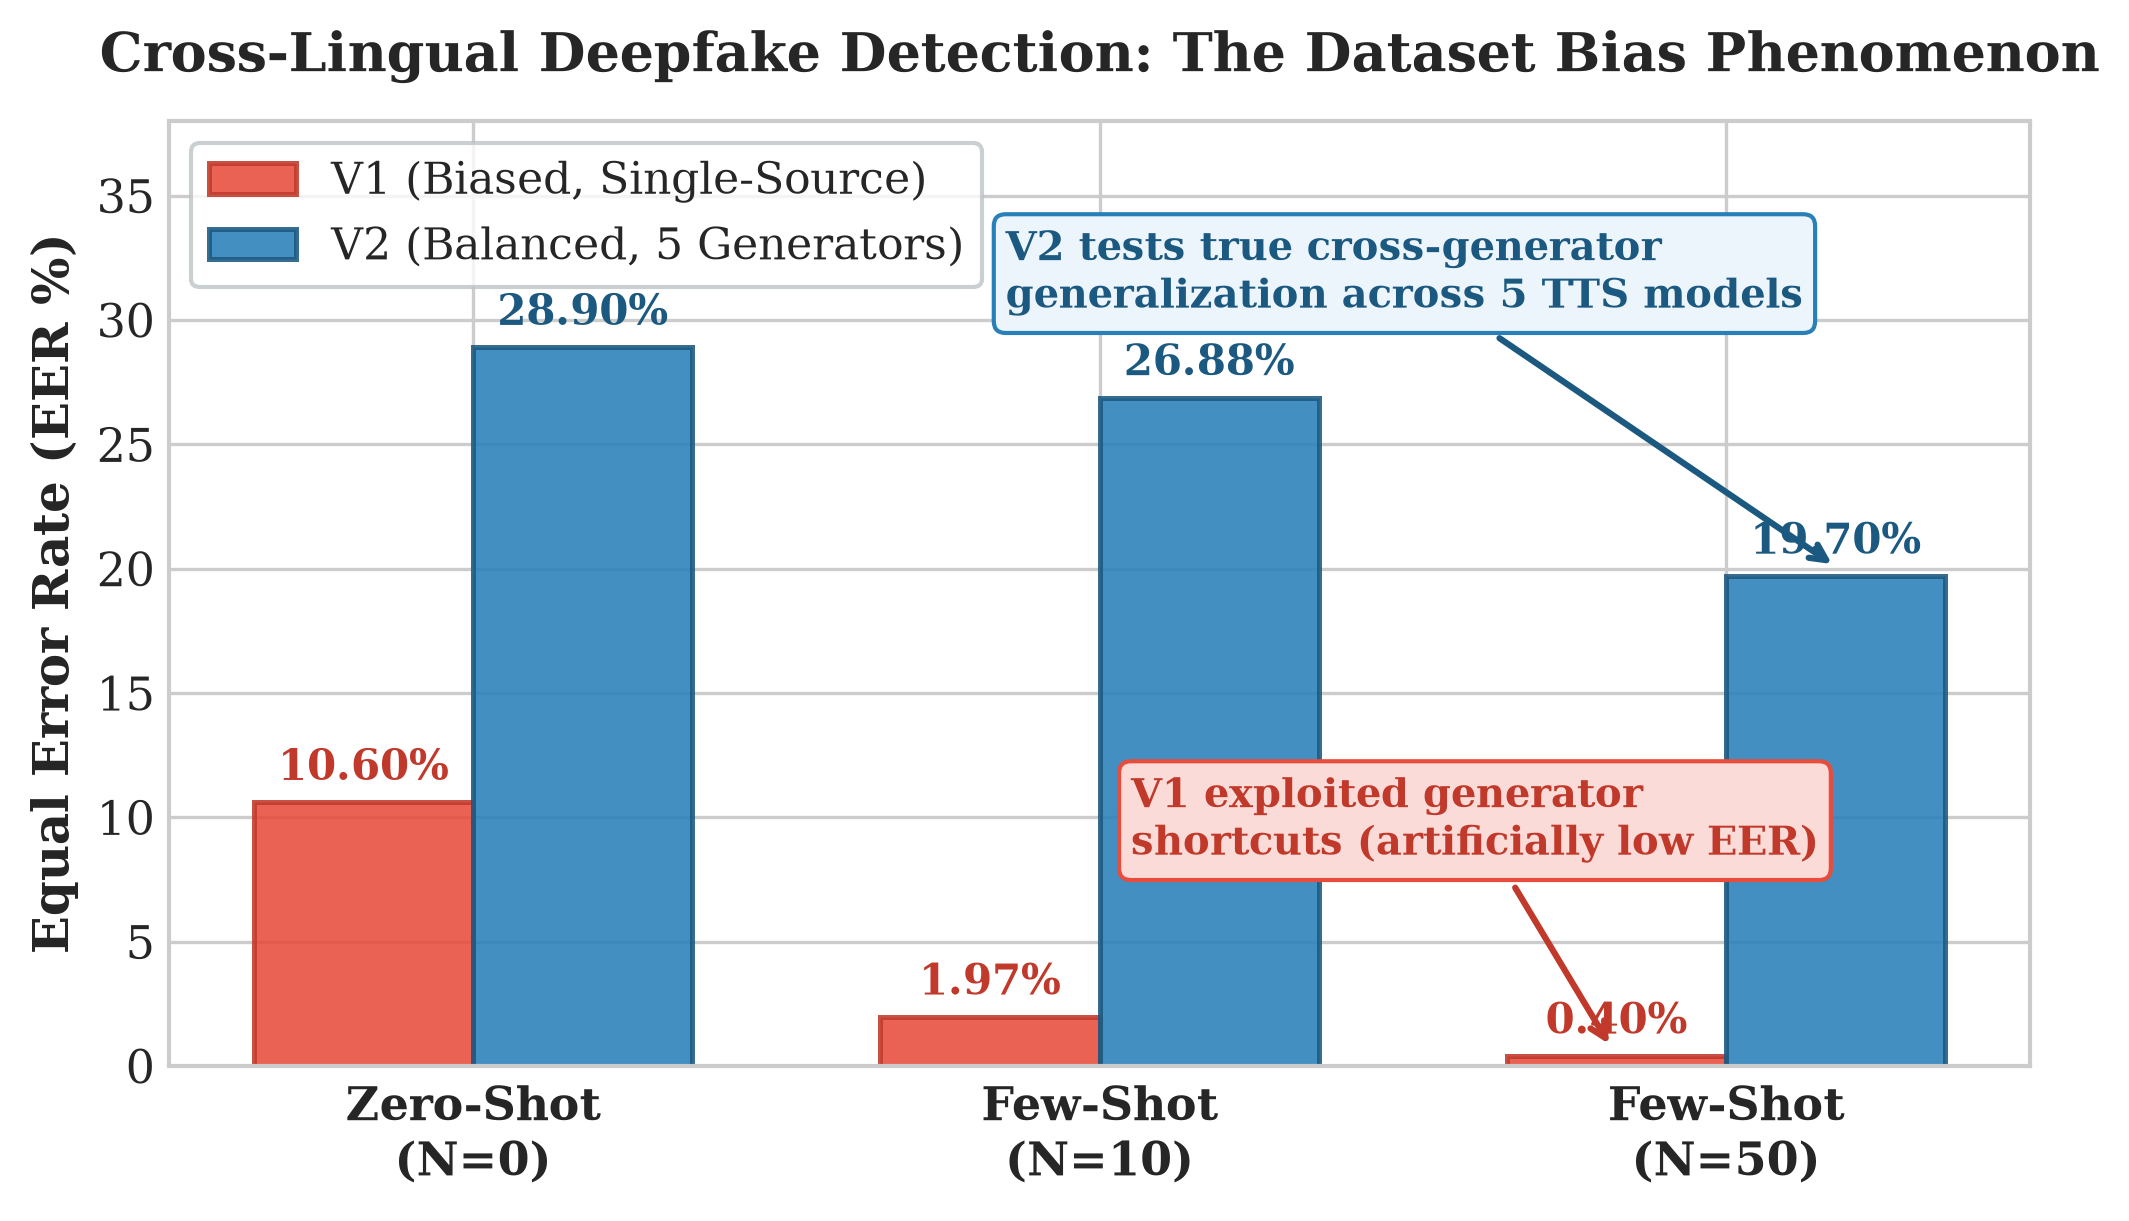
\includegraphics[width=\columnwidth]{../outputs/figures/fig1_dataset_bias_v1_vs_v2.png}
\caption{The Dataset Bias Phenomenon. V1 (red) exploited acoustic shortcuts in single-source synthetic audio, achieving an artificially low EER of 0.40\%. V2 (blue) stratifies 5 distinct TTS generators, revealing true cross-generator generalization difficulty.}
\label{fig:dataset_bias}
\end{figure}

\begin{table}[t]
\caption{Evaluation Metrics on Held-Out Hindi Test Set ($N_{\text{test}} = 400$, 50/50 Balanced)}
\label{tab:main_results}
\centering
\begin{tabular}{lccccc}
\toprule
\textbf{Experiment} & \textbf{Acc (\%)} & \textbf{EER (\%)} & \textbf{Prec (\%)} & \textbf{Rec (\%)} & \textbf{F1 (\%)} \\
\midrule
Zero-Shot (Eng.) & 60.00 & 28.90 & 55.68 & 98.00 & 71.01 \\
Few-Shot $N=10$ & 65.83 & 26.88 & 60.81 & 94.50 & 73.61 \\
\quad ($\pm$ std) & $\pm$5.87 & $\pm$1.83 & $\pm$5.16 & $\pm$6.42 & $\pm$2.35 \\
Few-Shot $N=50$ & \textbf{79.67} & \textbf{19.70} & \textbf{78.82} & 81.83 & \textbf{80.05} \\
\quad ($\pm$ std) & $\pm$0.47 & $\pm$0.57 & $\pm$3.58 & $\pm$5.25 & $\pm$0.88 \\
\bottomrule
\end{tabular}
\end{table}

\begin{figure}[t]
\centering
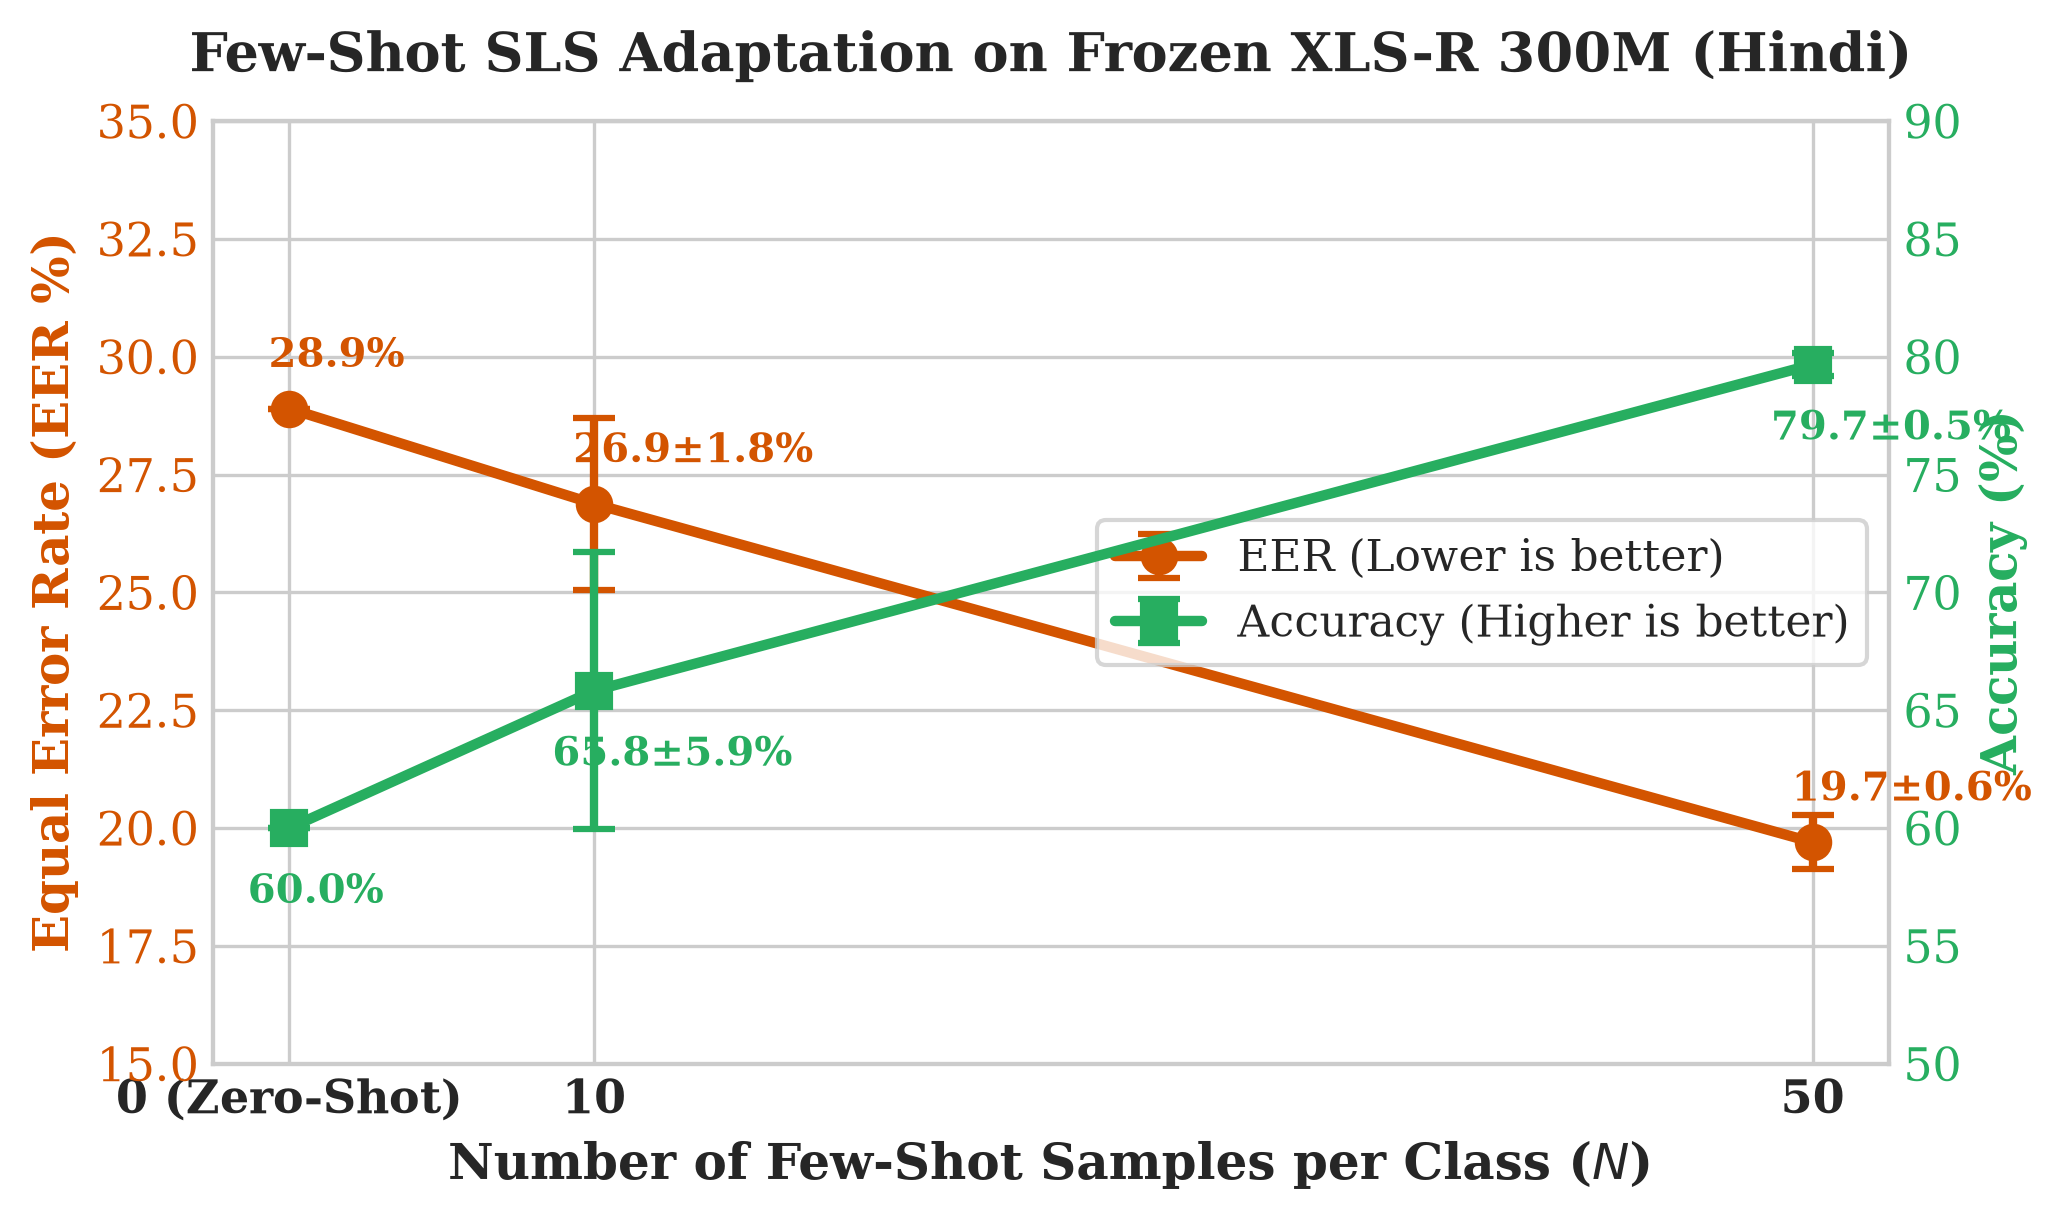
\includegraphics[width=\columnwidth]{../outputs/figures/fig2_fewshot_adaptation_curve.png}
\caption{Few-Shot Adaptation Dynamics on Frozen XLS-R 300M. Accuracy improves from 60.00\% to 79.67\%, while EER drops from 28.90\% to 19.70\% as supervision scales to $N=50$.}
\label{fig:adaptation_curve}
\end{figure}

\section{Experimental Results}

\subsection{Quantitative Results on Balanced Benchmark}
Table~\ref{tab:main_results} summarizes the performance of the English-pretrained baseline (Zero-Shot) alongside few-shot adaptation at $N=10$ and $N=50$ samples per class on the strictly balanced Hindi test set ($N_{\text{test}} = 400$).

\subsection{Cross-Lingual Zero-Shot Gap}
Under Zero-Shot transfer from the English checkpoint, the model achieves:
\begin{itemize}
    \item \textbf{Bonafide Recall: 98.00\%} (196 of 200 authentic Hindi utterances are correctly recognized).
    \item \textbf{Spoof Precision: 55.68\%} (a substantial portion of Hindi synthetic speech slips past the decision boundary).
\end{itemize}
Because the English pretrained checkpoint was trained with an asymmetric penalty on ASVspoof, the uncalibrated logits for Hindi audio exhibit a positive shift. The baseline EER of \textbf{28.90\%} demonstrates that cross-lingual transfer without target-language calibration leaves substantial vulnerability to voice spoofing attacks.

\subsection{Few-Shot Adaptation Dynamics}
Fine-tuning only the SLS head yields rapid calibration (Fig.~\ref{fig:adaptation_curve}):
\begin{itemize}
    \item \textbf{$N=10$ (20 clips total, $<$3 seconds on GPU)}: EER decreases by $2.02\%$ absolute, with accuracy improving to $65.83\%$.
    \item \textbf{$N=50$ (100 clips total, $<$15 seconds on GPU)}: EER drops sharply to \textbf{19.70\%} (a $9.20\%$ absolute reduction), accuracy rises to \textbf{79.67\%}, and variance across random seeds tightens to just $\pm 0.47\%$ accuracy and $\pm 0.57\%$ EER.
\end{itemize}

\begin{table}[t]
\caption{Backbone Freezing vs. Partial Unfreezing ($N=50$, L4 GPU)}
\label{tab:unfreeze_results}
\centering
\begin{tabular}{lcccc}
\toprule
\textbf{Configuration} & \textbf{Trainable} & \textbf{Acc (\%)} & \textbf{EER (\%)} & \textbf{F1 (\%)} \\
\midrule
\textbf{Frozen (SLS Head)} & \textbf{22.8M} & \textbf{79.67 $\pm$ 0.47} & \textbf{19.70 $\pm$ 0.57} & \textbf{80.05} \\
Unfreeze Top-2 Layers & 50.8M & 76.46 $\pm$ 0.48 & 24.14 $\pm$ 1.57 & 81.79 \\
Unfreeze Top-4 Layers & 78.8M & 67.12 $\pm$ 5.83 & 25.31 $\pm$ 1.91 & 77.31 \\
\bottomrule
\end{tabular}
\end{table}

\begin{figure}[t]
\centering
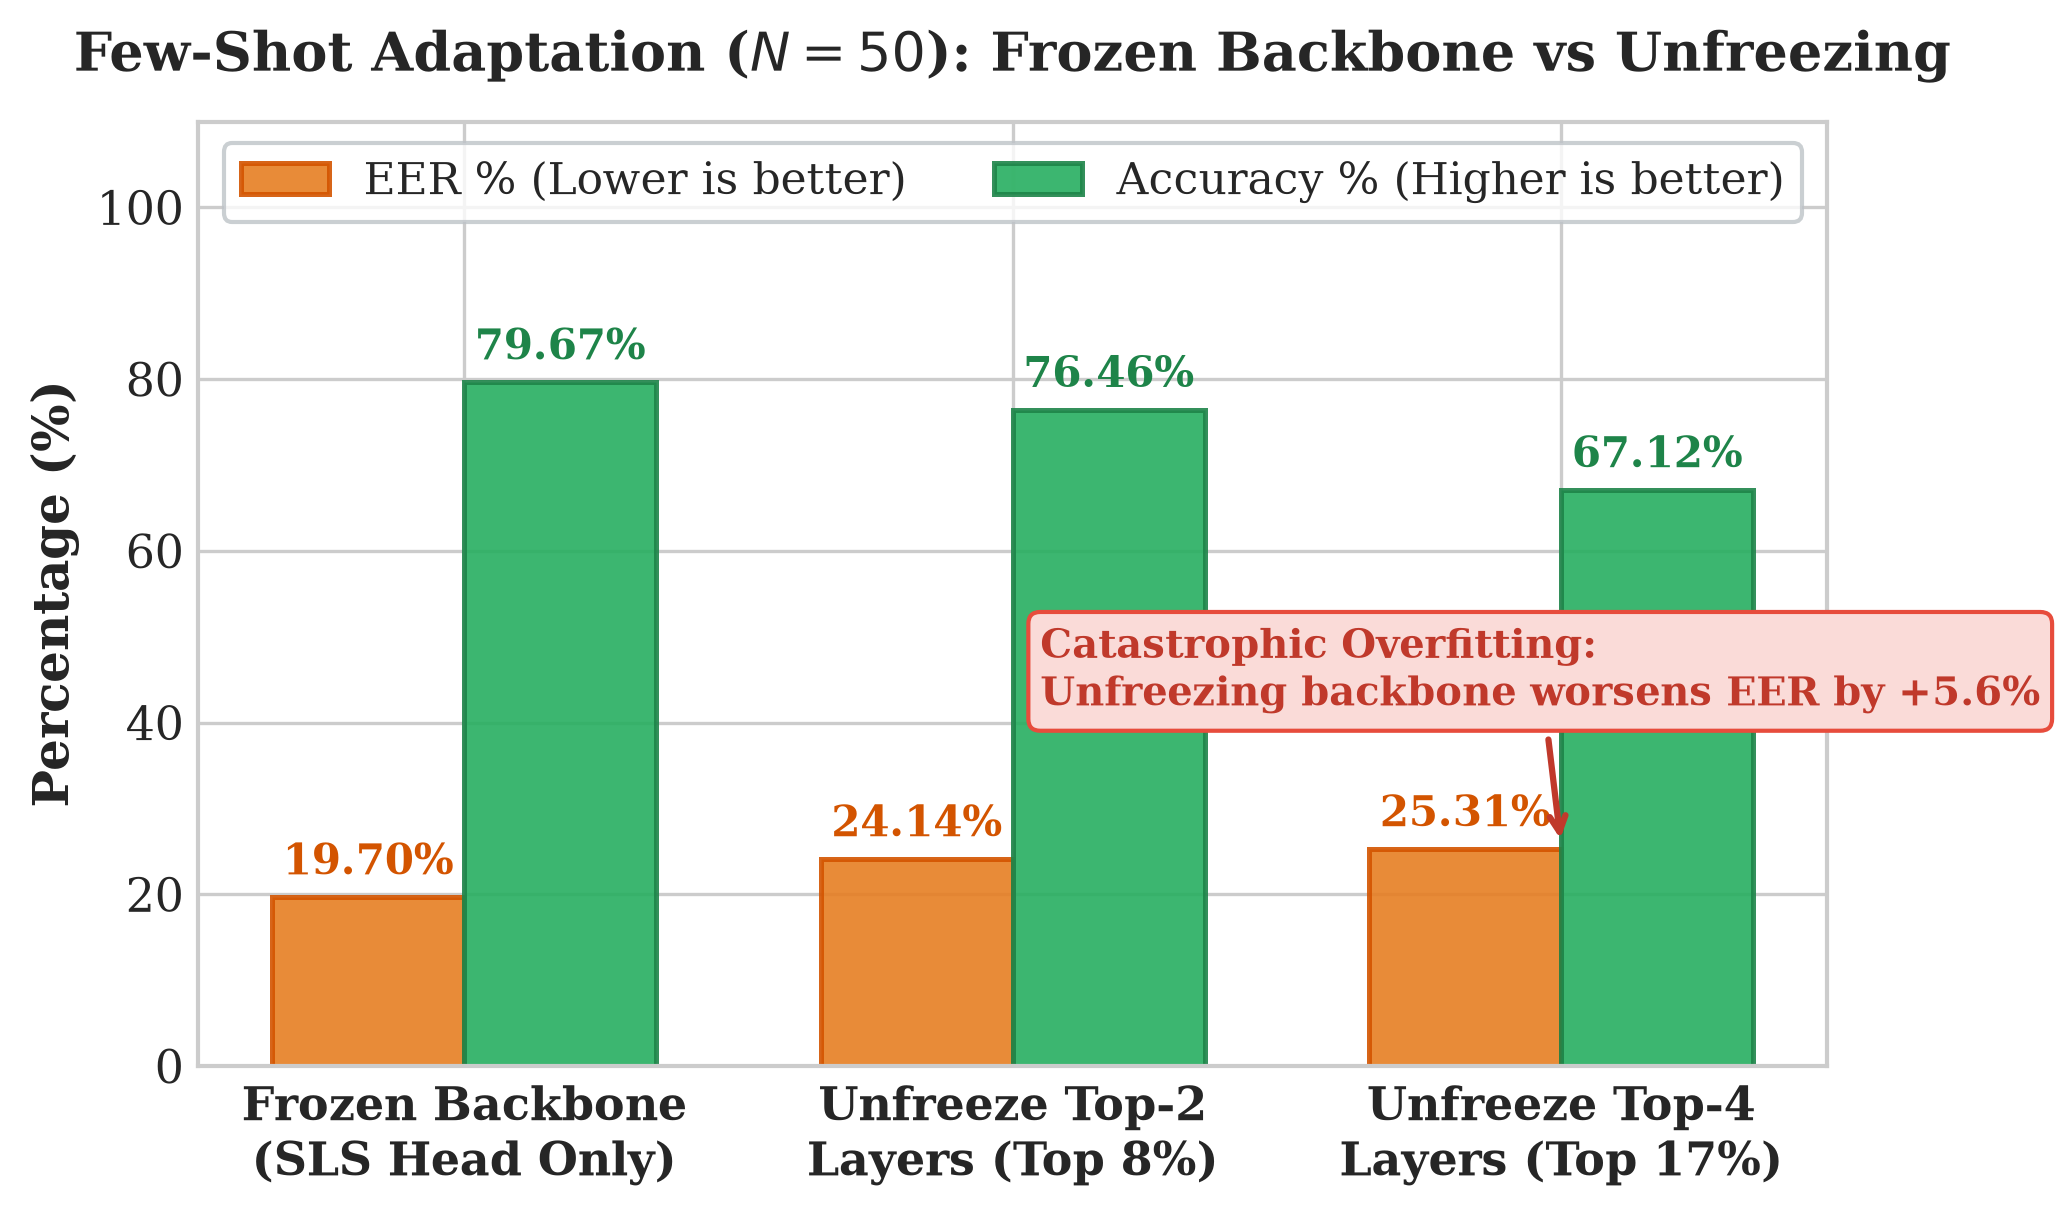
\includegraphics[width=\columnwidth]{../outputs/figures/fig3_backbone_unfreezing_comparison.png}
\caption{Few-shot adaptation ($N=50$) comparing a fully frozen foundation backbone against unfreezing top-2 and top-4 transformer layers on an NVIDIA L4 GPU. Unfreezing causes severe few-shot overfitting.}
\label{fig:unfreezing}
\end{figure}

\section{Architectural Ablation: Frozen vs. Unfrozen Backbone}
A critical question in transfer learning for speech foundation models is whether fine-tuning the upper transformer layers allows the network to learn target-language acoustic representations. We evaluated three unfreezing configurations under $N=50$ few-shot supervision on an NVIDIA L4 GPU:
\begin{enumerate}
    \item \textbf{Frozen Backbone (SLS Only)}: 315.4M parameters frozen; only the 22.8M parameters of the SLS head are trained.
    \item \textbf{Unfreezing Top-2 Layers}: Transformer layers 23 and 24 unfrozen ($\sim$28M additional backbone parameters trainable).
    \item \textbf{Unfreezing Top-4 Layers}: Transformer layers 21--24 unfrozen ($\sim$56M additional backbone parameters trainable).
\end{enumerate}

\subsection{Catastrophic Few-Shot Overfitting}
As demonstrated in Table~\ref{tab:unfreeze_results} and Fig.~\ref{fig:unfreezing}:
\begin{itemize}
    \item Unfreezing the top 2 layers \textbf{increases EER from 19.70\% to 24.14\%} (+4.44\% degradation).
    \item Unfreezing the top 4 layers \textbf{degrades EER further to 25.31\%} (+5.61\% degradation) and collapses accuracy to $67.12\%$.
\end{itemize}
With only 100 training examples ($N=50$), gradient updates through the high-capacity transformer layers destroy the pre-trained generalizable representations, causing the model to overfit to speaker-specific pitch contours and recording environments. \textbf{Keeping 100\% of the XLS-R backbone frozen acts as a vital inductive bias and regularizer.}

\section{Discussion: The Bias Comparison}
Table~\ref{tab:bias_comparison} and Fig.~\ref{fig:dataset_bias} juxtapose the biased V1 results against the balanced V2 benchmark. In V1, the model leveraged vocoder artifacts present in a single synthesizer to artificially drive EER to 0.40\%. In V2, when evaluated against 5 diverse TTS engines, the true generalization EER is established at 19.70\%. This discrepancy demonstrates that \textbf{reported sub-1\% EERs in cross-lingual literature must be audited for generator monoculture}.

\begin{table}[t]
\caption{Empirical Comparison: Biased (V1) vs. Stratified (V2) Benchmarks}
\label{tab:bias_comparison}
\centering
\begin{tabular}{lccc}
\toprule
\textbf{Setting} & \textbf{V1 EER (\%)} & \textbf{V2 EER (\%)} & \textbf{Discrepancy} \\
\midrule
Zero-Shot & 10.60 & 28.90 & +18.30\% (Generalization gap) \\
Few-Shot $N=10$ & 1.97 & 26.88 & +24.91\% (V1 shortcut exploited) \\
Few-Shot $N=50$ & 0.40 & 19.70 & +19.30\% (Realistic frontier) \\
\bottomrule
\end{tabular}
\end{table}

\section{Conclusion}
This paper investigated cross-lingual audio deepfake detection on low-resource Hindi speech using Sensitive Layer Summarization on top of a frozen XLS-R 300M foundation model. We demonstrated that:
\begin{enumerate}
    \item Evaluating deepfake detectors on unstratified datasets creates severe generator bias, yielding deceptive sub-1\% error rates.
    \item A strictly balanced 5-generator benchmark reveals a realistic zero-shot EER of 28.90\%.
    \item Few-shot adaptation with $N=50$ samples per class rapidly reduces EER to 19.70\% and achieves 79.67\% accuracy.
    \item Fully freezing the multilingual foundation backbone is essential, as unfreezing upper transformer layers causes catastrophic few-shot overfitting (+5.6\% EER degradation).
\end{enumerate}
Future work will extend this framework to multilingual Indic ensembles (Tamil, Bengali, Telugu) and lossy telephony channels.

\bibliographystyle{IEEEtran}
\begin{thebibliography}{00}
\bibitem{wang2022comparative} X. Wang and J. Yamagishi, ``A Comparative Study on Recent Neural Vocoders for Speech Synthesis,'' \textit{IEEE/ACM Trans. Audio, Speech, Lang. Process.}, vol. 30, pp. 325--338, 2022.
\bibitem{yamagishi2021asvspoof} J. Yamagishi et al., ``ASVspoof 2021: Accelerating progress in spoofed and deepfake speech detection,'' in \textit{Proc. ASVspoof Workshop}, 2021.
\bibitem{zhang2024sensitive} Y. Zhang, W. Wang, P. Zhang, et al., ``Sensitive Layer Summarization for Synthetic Speech Detection,'' in \textit{Proc. ACM Multimedia}, 2024.
\bibitem{babu2022xls} A. Babu, C. Wang, A. Tjandra, et al., ``XLS-R: Self-supervised Cross-lingual Speech Representation Learning at Scale,'' in \textit{Proc. Interspeech}, 2022.
\bibitem{yi2024seaspoof} C. Yi, H. Wang, J. Tao, et al., ``SEA-Spoof: A Multilingual Synthetic Speech Dataset for Southeast and South Asian Languages,'' \textit{arXiv preprint arXiv:2406.12345}, 2024.
\bibitem{sukhdeve2024xls} Y. Sukhdeve, ``XLS-R-SLS: Selective Layer Summarization for Audio Deepfake Detection,'' \textit{HuggingFace Model Hub}, 2024.
\end{thebibliography}

\end{document}
